% status: 0
% chapter: TBD

\title{GraphQL, Advancing APIs}

\author{Averill Cate, Jr}
\affiliation{%
  \institution{The University of Indiana}
  \streetaddress{}
  \city{Bloomington} 
  \state{Indiana} 
  \postcode{47408}
}
\email{acate@iu.edu}

% The default list of authors is too long for headers}
\renewcommand{\shortauthors}{A. Cate, Jr}

\begin{abstract}
We are in the information age.  Possibly, the information overload age.
Data are the commodity of this technological era.  A significant number, if not
most of the world's industries are dependent on the internet and the exchange
of data.  It is reasonably safe to assume that how data are exchanged is
an important to understand.  Understanding data services have been changing
over time may be as vital as development of new tools and methods for data
exchange.  This paper will describe changes in data service methods and 
technologies and assert possible reasons why those changes are occurring and 
why those changes may improve how data are exchanged as we progress further 
into the information age.
\end{abstract}

\keywords{hid505, GraphQL, Web Services, Cloud, Computing}

\maketitle

\section{Introduction}
Although data services and data exchange long pre-date the early 2000's.  The
volume of work that pre-dates 2000 would require volumes to adequately describe.
For clarity, this paper focuses on data services technologies that have emerged
since 2000 and the advent of Web 2.0 and in particular the data mining and
data sciences explosion that is taking place across the globe.

``Web services evolved from the Remote Procedure Call (RPC) mechanism.``\cite{Kalin2009}.  
The development of web services is meant to address a distributed computing 
environment, where data might be stored on one system, applications consuming 
or processing that data might be stored on a second system and clients that 
render data are on systems like desktop computers, mobile devices or other 
machines further process that data.  All of these systems are linked together, 
typically via some sort of network and an RPC system provides a mechanism so 
that both the data and procedures that can be used on that data are 
discoverable\cite{Kalin2009}.

SOAP and XML, REST and JSON have been part of the progression of the development
of web services and web Application Programming Interfaces (API).  Some might 
say that the development of each has revealed something new that has lead to 
the next technological advancement in data services and data.  After the 
development of a new technology we also discover limitations of that 
technology, which in-turn leads to the next technological advancement.  For 
example, not long after SOAP and XML became primary tools in web API 
development, some people began to notice the difficulty in reading XML data in 
cases where developers need to confirm data requests or data responses.  One 
might argue that using XML as the data packet could have been an over extension 
of the use of XML in web services.  In the mid to late 2000s, REST and JSON 
based web services began to take hold.  JSON may have been a better fit for 
web services and data mining because formatting data to comply with a JSON 
data format focuses more on the data itself than describing the data like XML 
does.  If true, and we concede the format of JSON data rendered for situations 
where developers are trying to test web services and the rendered data are 
easier to read then JSON may have been the next logical step in the evolution 
of web services.  

This paper will briefly describe two import exchange protocols, SOAP and REST.  
Next the paper will compare XML, a data format used in SOAP, with two data
formats used in REST, JSON, and GraphQL.  SOAP and REST are not the only
protocols that currently exist.  Nor are XML, JSON, and GraphQL the only data
formats that exist.  However, both protocols and all three formats are widely
used in academia and industry today and merit discussion.  

\section{SOAP and XML}
SOAP is a XML-based data exchange protocol\cite{Quaine2007}.  SOAP stands for
``Simple Object Access Protocol``\cite{Microsoft2018}.  SOAP is a lightweight
protocol that, simply stated, is extensible and designed to facilitate the
exchange of structured data between disparate systems\cite{Microsoft2018}.
Extensible Markup Language (XML) is the structured data format that has been
used in conjunction with SOAP for data services\cite{Walsh1998}.  SOAP and XML
are still widely used today.  In some cases, due to legacy systems and security
concerns SOAP and XML are required for the use and development of data services.
An example of XML is shown in Figure~\ref{f:xml-example}\cite{WikipidiaXML1028}.
\begin{figure}[!ht]
  \centering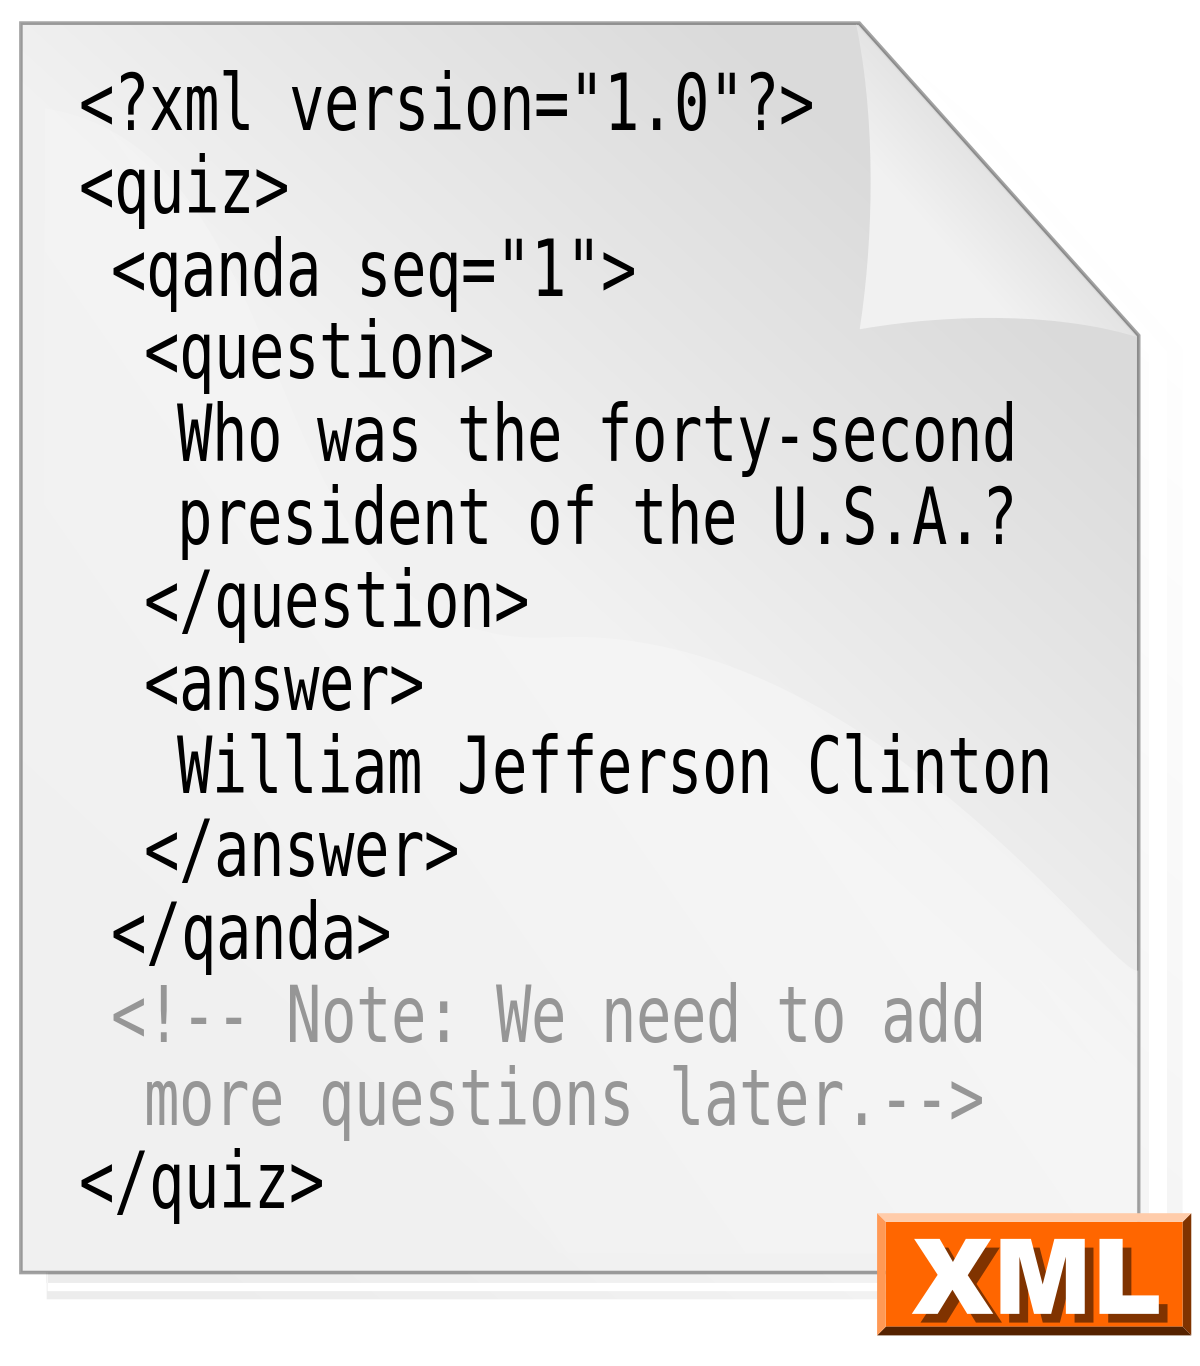
\includegraphics[width=\columnwidth]{images/xml-example.png}
  \caption{SOAP/XML Example}\label{f:xml-example}
\end{figure}
An important point to note is, XML is a markup language, which can be
interpreted as a meta-language.  XML serves to not only contain the data it
delivered, but it also describes the data\cite{Aihkisalo2012}.

Figure~\ref{f:wsdl-example}\cite{mycodde2016} is an example of the type of
interface developers and web service data consumers had to understand in order
to work effectively with SOAP/XML based web services.  
\begin{figure}[!ht]
  \centering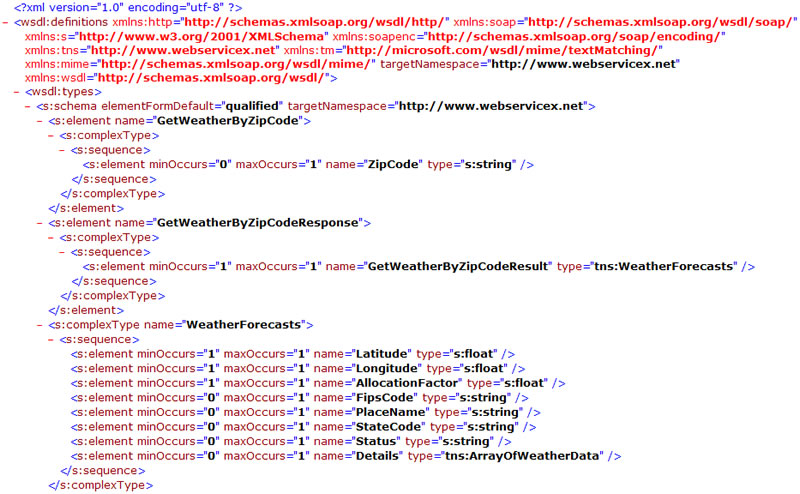
\includegraphics[width=\columnwidth]{images/wsdl-example.jpg}
  \caption{WSDL Example}\label{f:wsdl-example}
\end{figure}
Anyone trying to read the WSDL document had to not only understand the nuances 
of things like XML, name-spacing, but also had to be able to understand how the 
web service's operations were defined in the WSDL document.

\section{REST and JSON}
Pautasso\cite{Pautasso2008} define REST as Representational State
Transfer.  REST was designed by Roy Fielding as part of his doctoral
dissertation while attending the University of California, Irvine\cite{Fielding2000}.
Fielding developed REST in order to propose a framework for and architecture
that can be used in ``network-based application software``\cite{Fielding2000}.
Fielding's work on REST occurred around 2000, but it has only been in the last
few years that we have seen the widespread implementation of REST.
Figure~\ref{f:rest-example} we show an example of a REST/JSON data packet.  
\begin{figure}[!ht]
  \centering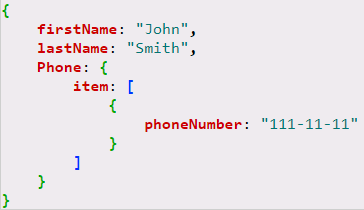
\includegraphics[width=\columnwidth]{images/json-rest-example.png}
  \caption{REST/JSON Example}\label{f:rest-example}
\end{figure}
The example could be the output from a query to a RESTful web service or the 
input to be delivered to a RESTful web service that is meant to create our update 
data.  JSON in comparison to XML is not a markup language.  In comparison to XML, 
JSON is the data with some defining attributes, but it his little, if any, 
meta-data that describe the data itself.  As an example, a JSON data packet 
might have a list of users where each user object or item has a first name 
attribute, last name attribute and an email address attribute with values for 
each of those attributes, but the data packet itself, does not describe the data 
format.  REST and JSON have also leant themselves towards the development of 
web-based APIs.

Figure~\ref{f:swaggerui-example}\cite{swaggerio2018} is example of a REST/JSON web service
interface.  
\begin{figure}[!ht]
  \centering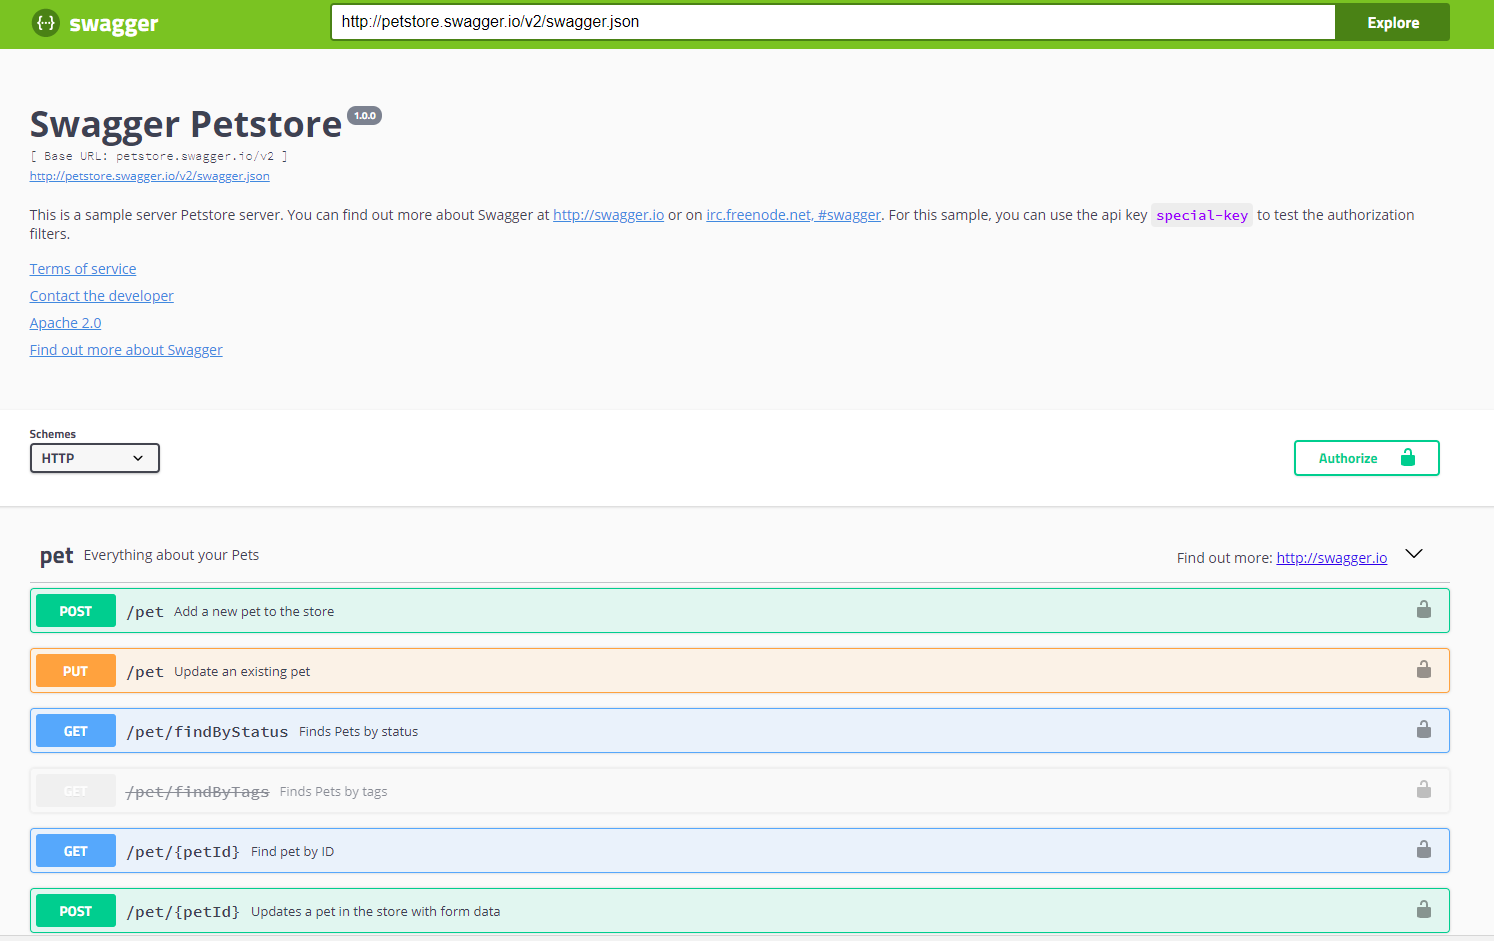
\includegraphics[width=\columnwidth]{images/swaggerui.png}
  \caption{Swagger UI Example}\label{f:swaggerui-example}
\end{figure}
In comparison, it seems easier to understand not only the procedures
or methods the service provides, but as Figure~\ref{f:swaggerui-expansion}\cite{swaggerio2018}
demonstrates, it is easier to understand the data types required for the services input
parameters and resulting output data packets.  
\begin{figure}[!ht]
  \centering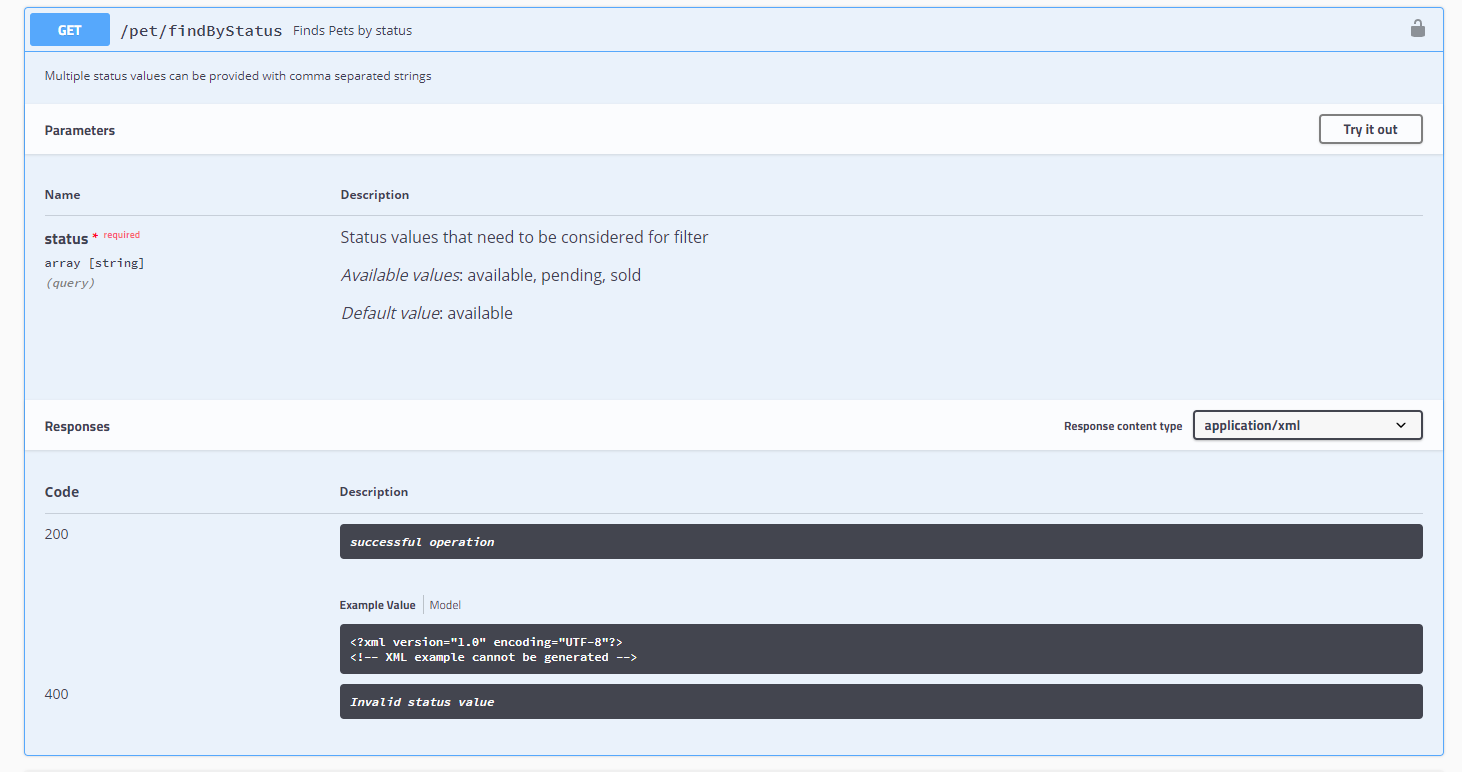
\includegraphics[width=\columnwidth]{images/swaggerui-expansion.png}
  \caption{Swagger UI Expanded}\label{f:swaggerui-expansion}
\end{figure}
However, Figure~\ref{f:swagger-resp}\cite{swaggerresp2018} provides an example 
of service response from a REST/JSON based service and although, visually, 
easier to understand compared XML.  
\begin{figure}[!ht]
  \centering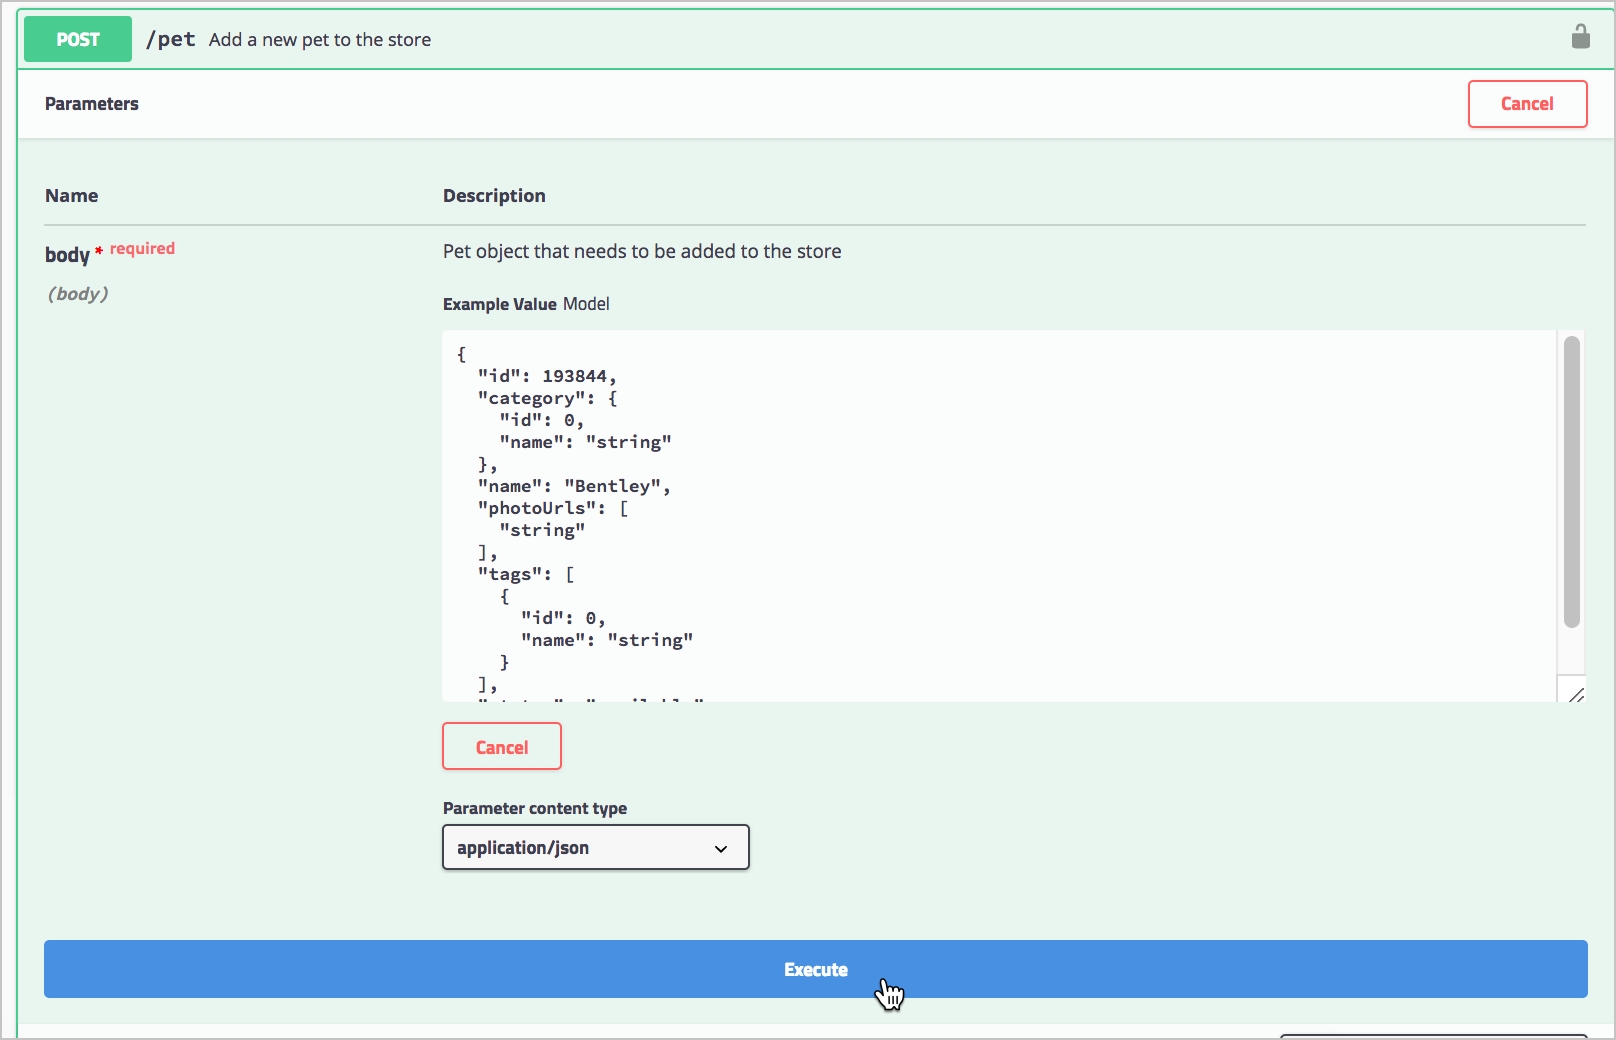
\includegraphics[width=\columnwidth]{images/swaggerui_execute.png}
  \caption{Swagger UI Response}\label{f:swagger-resp}
\end{figure}
It can be challenging to understand the relationships between the data set's 
components.

\section{GraphQL}
``GraphQL is a query language constructed to facilitate the development of APIs``\cite{FacebookGraphQL2018}.
GraphQL is meant to provide a complete and understandable description of the
data in an API as well as allowing clients to ask for exactly what data is 
needed and nothing more than that\cite{FacebookGraphQL2018}.  GraphQL was 
developed by Facebook to address Facebook's need for having an API that could 
retrieve and describe all of Facebook's data while keeping the API simple to 
learn and use\cite{Byron2015}.

An issue with both SOAP and REST based services is that once a remote
procedure is implemented both inputs and outputs are fixed.  In other words,
a developer has to create the appropriate inputs and its required input values
for an RPC call.  The remote procedure produces a resulting data set with the
exact same output fields each time.  For example, the developer instantiates an
API call to retrieve a list of all users.  A single user has three attributes,
first name, last name, and email address.  The resulting user list always has
all three attributes.  However, what if the developer wants the same list of
users, but only wants the first and last name attributes of each user.  GraphQL
provides that flexibility.

Figure~\ref{f:github-graphql-1} shows an example of a GraphQL query and the
results using GithHub.com's GraphQL API.  
\begin{figure}[!ht]
  \centering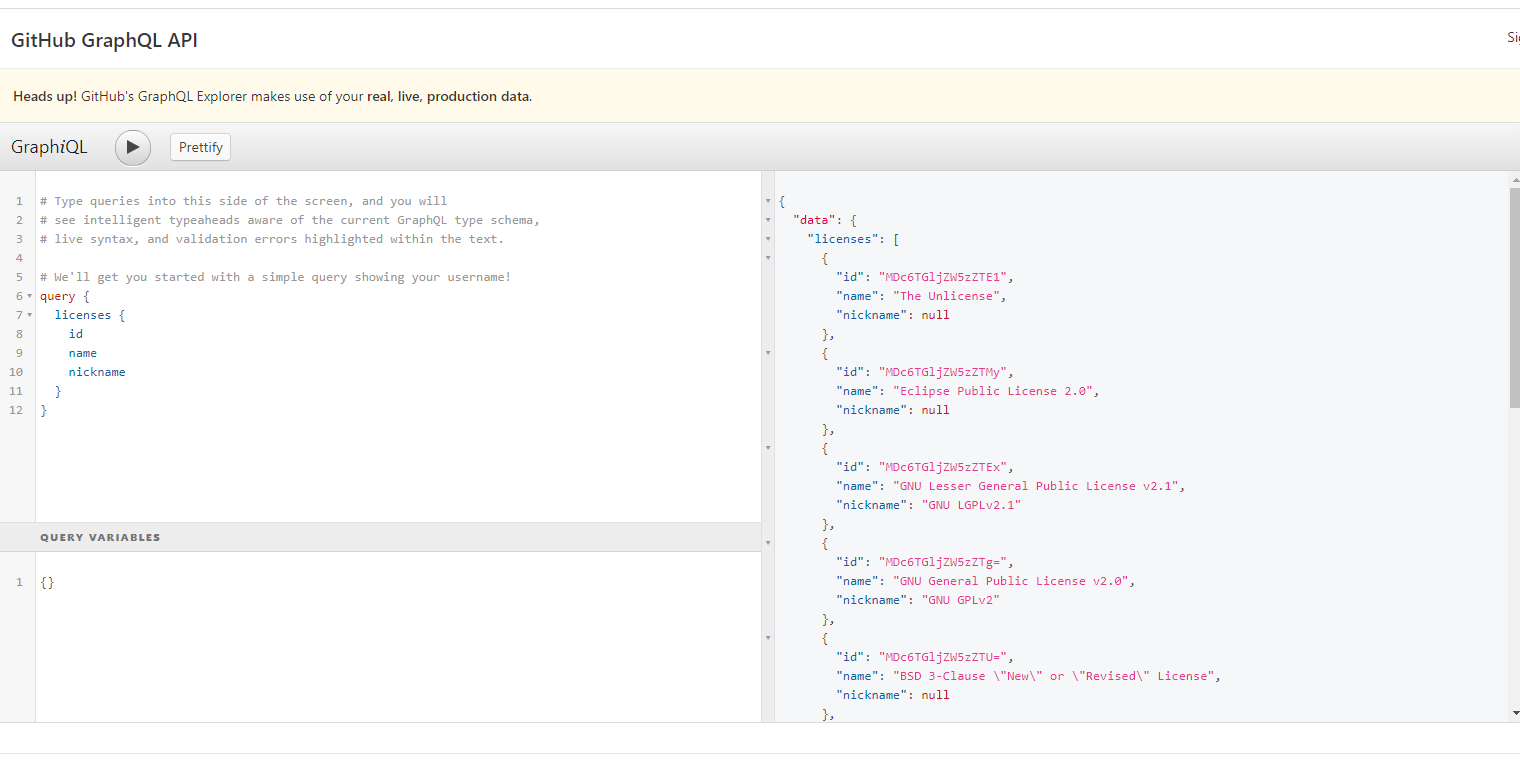
\includegraphics[width=\columnwidth]{images/github-graphql-1.png}
  \caption{GitHub GraphQL Licenses Query}\label{f:github-graphql-1}
\end{figure}
Figure~\ref{f:github-graphql-2} is an
example of using GitHub's same GraphQL API, but requesting the list of licenses
excluding the nickname field.
\begin{figure}[!ht]
  \centering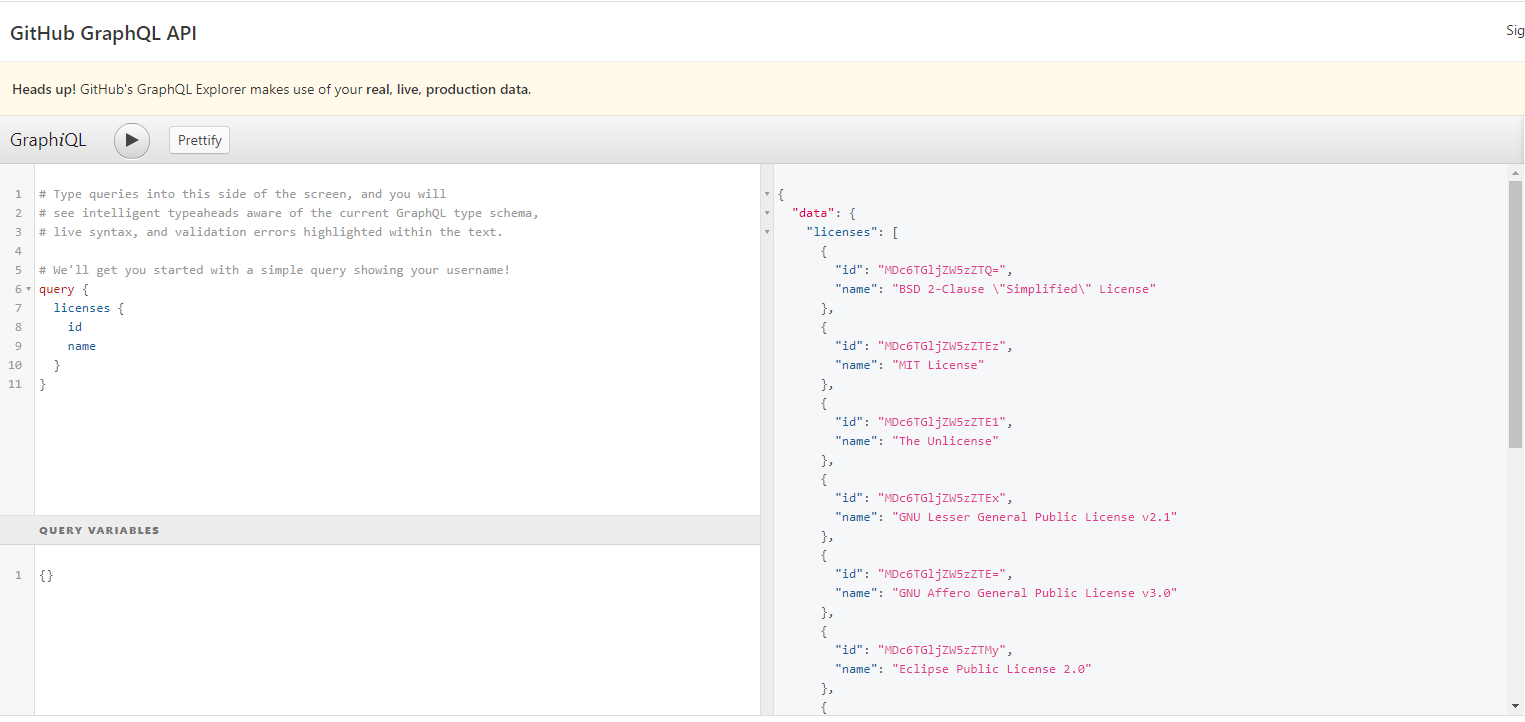
\includegraphics[width=\columnwidth]{images/github-graphql-2.png}
  \caption{GitHub GraphQL Licenses Query Without Nickname Field}\label{f:github-graphql-2}
\end{figure}

A second issue that has been a challenge to manage in SOAP and REST based APIs
has been versioning.  In a REST API, an endpoint for requesting users might look
like:
\begin{verbatim}http://somedomain.com/api/v1.0/users \end{verbatim}
Over time the API might need to evolve and the next version of the equivalent
user call might produce a data set that has slightly different attributes for
the user. The new endpoint might look like:
\begin{verbatim}http://somedomain.com/api/v2.0/users \end{verbatim}
This versioning structure requires work to make sure the new version of the API
is documented.  Effort is also required to make sure the previous version of the
API is documented and there is good communication with API consumers so they
know there are multiple versions of the API and the differences between those
versions.  Simply stated, GraphQL does not create this situation.  If the domain
model for the user object changes to include a new field (e.g., phone number),
then the new field can be added to the model.  The GraphQL query schema can be
adjusted for new field and anything that consumes that already accesses that 
GraphQL query will continue to work.

A third issue that GraphQL addresses that can be viewed as a challenge in SOAP 
or REST services is accessing related resources in single requests\cite{FacebookGraphQL2018}.  
Typically in REST or SOAP, if a user object had a one-to-many relationship to 
an address object and an API consumer wanted to get a user's address data then 
multiple calls have to be created to retrieve the related resources 
(i.e., addresses).  Also, the API developers have to develop and maintain 
multiple API endpoints (i.e., user endpoint, addresses endpoint).

A fourth feature that GraphQL offers that relates back to it being a single 
(url) resource is, efficiency.  Micro-services and a micro-service based 
architecture has emerged as robust and popular format for delivering web 
services.  Technically, the goal of a micro-service is to keep the service small 
and easy to maintain. REST based services tend to require multiple endpoints 
that can be used for typical Create, Read, Update Delete (CRUD) operations.  
GraphQL's single endpoint means that all CRUD operations are handled by a single 
endpoint making the resources required to build and run the service smaller.

\section{Conclusion}
There have been very notable advances in data and service delivery since the 
advent of the Internet and the Internet's integration into industry.  At the 
same time we are seeing incredible increases in the amounts and demands for 
data that are used in almost every business and academic sector.  With these 
changes we see enhancement to the tools used to deliver the data and the 
services.  

In the early 2000s, we saw data delivery handled via tools like SOAP and XML 
where XML data packets not only contained the data, but contained meta-data 
that described the data in the packet.  This required service users to have to 
develop an understanding of the data and the domain at the same time.  This 
would not have necessarily been a bad thing, but it would have required more 
effort.

Between approximately 2005 and 2015 we have seen a wider acceptance and 
implementation of REST and JSON based web services.  Using JSON as the format 
for structuring data has lead to possibly cleaner and easier to understand 
data packets while leaving the metadata for those packets and services as part 
of the APIs documentation.  However, this still means that someone has to 
develop and maintain the documentation (metadata) and that service consumers 
have to expend effort to stay aware of changes to the services being consumed 
in case a change occurs that might affect the clients accessing those services.

A slightly more rigorous way to gage whether GraphQL has traction for becoming 
reliable part of web and data services infrastructure is to examine who is 
using GraphQL.  According to the GraphQL website (graphql.org/users/), major 
companies like Coursera, Facebook, GitHub, Intuit, Neo4j, Shopify, Twitter 
and Yelp are using GraphQL\cite{GraphQLUsers2018}.  Assuming that most of these 
organizations investigate and research new technological tools before making 
the tools part of their infrastructure, it may be reasonable to assume that 
GraphQL has notable viability.

Figure~\ref{f:network-response}\cite{VzquezIngelmo2017ImprovingTO} also 
provides data that could support the choice of using GraphQL as a part of a 
services system architecture.  
\begin{figure}[!ht]
  \centering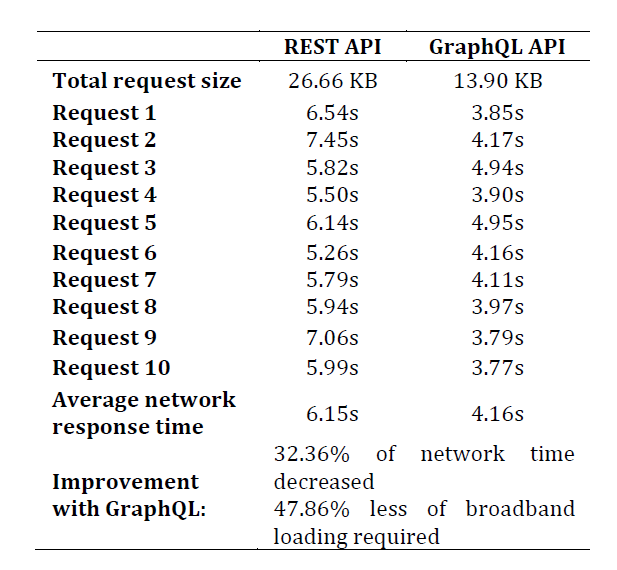
\includegraphics[width=\columnwidth]{images/network-response-times.png}
  \caption{GraphQL and REST Network Response Times}\label{f:network-response}
\end{figure}
The table indicates that GraphQL performance may be better than REST.  GraphQL 
has an almost 50 percent performance increase.  Serious architecture related 
decisions would require checking the constraints of the test and repeating the 
tests for verification.

Finally, in approximately 2016, developers at Facebook seemed to have 
developed the next step forward in service and data delivery by addressing some 
of the weaknesses in SOAP/XML and REST/JSON by creating and publishing GraphQL.
Because GraphQL is a query language the structure of the query and the language 
used to create a query have, what seems to be, a more intuitive fit to the data 
domain.  This may allow service developers and consumers to work with the 
services without having to spend time in trying to understand the underlying 
mechanisms used to deliver the services and the data.  GraphQL requires a 
single endpoint for service access therefore minimizing the need for developers 
to maintain and document multiple endpoints and/or having to version the API.  
Lastly, API consumers will be able to use a query format that matches more 
closely the resulting data set produced from query requests, which could help 
facilitate understanding the data and services provided by the API.

\begin{acks}

  The author would like to thank Dr.~Gregor~von~Laszewski for his
  support and suggestions to write this paper.

\end{acks}

\bibliographystyle{ACM-Reference-Format}
\bibliography{report} 
